\chapter{Gestión de Memoria}

En un sistema \textit{monoprogramado}, la memoria principal se divide en dos partes: una para el sistema operativo y otra para el único programa en ejecución. En un sistema \textit{multiprogramado}, la memoria de usuario debe compartirse dinámicamente entre varios procesos. Esta tarea es responsabilidad del \textit{sistema operativo} y se conoce como \textit{administración de memoria}.

Una buena administración de memoria permite mantener suficientes procesos listos para ejecutar, evitando que el procesador permanezca inactivo mientras otros procesos esperan operaciones de E/S.

\section{Requisitos de la administración de memoria}

Un sistema de administración de memoria debe satisfacer los siguientes requisitos:
\begin{enumerate}
  \item Reubicación.
  \item Protección.
  \item Compartición.
  \item Organización lógica.
  \item Organización física.
\end{enumerate}

\subsection{Reubicación}

En un sistema multiprogramado, un proceso puede cargarse en cualquier región de memoria e incluso ser trasladado durante su ejecución (por ejemplo, mediante \textit{swapping}). Por ello, las direcciones utilizadas por el programa no pueden corresponder directamente a direcciones físicas.

\begin{figure}[!ht]
  \centering
  \begin{tikzpicture}[>=Stealth,font=\scriptsize]
    \fill[fill=gray!20] (0.1,-0.1) rectangle (2.1,5.4);
    \draw[fill=white!94!blue!93!green] (0,0) rectangle node{Pila} (2,1);
    \draw[fill=white!94!blue!93!green] (0,1) rectangle node{Datos} (2,3);
    \draw[fill=white!94!blue!93!green] (0,3) rectangle node{Programa} (2,5);
    \draw[fill=white!94!blue!93!green] (0,5) rectangle node{PCB} (2,5.5);
    \draw[->] (1.7,4.7) -- (2.6,4.7) -- node[right,text width=1.4cm]{Instrucción de salto} ++(0,-.7) -- (2,4);
    \draw[->] (1.7,3.4) -- (2.6,3.4) -- node[right,text width=1.4cm]{Referencia a datos} ++(0,-1) -- (2,2.4);
    \draw[<-] (0,1) -- ++(-.7,0) node[left,text width=2cm,draw,rectangle]{Cima actual de la pila};
    \draw[<-] (0,5) -- ++(-.7,0) node[below left,text width=2.3cm,draw,rectangle]{Punto de entrada del programa};
    \draw[<-] (0,5.5) -- ++(-.7,0) node[above left,text width=2.3cm,draw,rectangle]{Bloque de control de proceso};
    \draw[thick,->] (-1,3.5) --node[left,text width=2cm]{Incremento de direcciones} (-1,2.5);
  \end{tikzpicture}
  \caption{Requisitos de direccionamiento de un proceso.}
  \label{fig:direccionamiento_proceso}
\end{figure}

La figura \ref{fig:direccionamiento_proceso} muestra una imagen de un proceso. Para simplificar, supongamos que dicha imagen ocupa una región contigua de la memoria principal. El sistema operativo necesita conocer la ubicación del PCB y de la pila de ejecución, además del punto de entrada para comenzar la ejecución del programa de ese proceso. Como el sistema operativo administra la memoria y se encarga de traer el proceso a la memoria principal, estas direcciones son fáciles de obtener.

Además, el procesador debe manejar las referencias a memoria dentro del programa: las instrucciones de salto incluyen la dirección de la siguiente instrucción a ejecutar; y las instrucciones de acceso a datos contienen la dirección del byte o palabra de datos referenciado. 

De alguna manera, el hardware y el sistema operativo deben traducir las referencias a memoria que aparecen en el código del programa a direcciones físicas reales, reflejando la ubicación actual del programa en la memoria principal, permitiendo que el proceso se ejecute independientemente de su ubicación en memoria.

\subsection{Protección}

Cada proceso debe estar aislado de los demás para impedir accesos no autorizados, ya sean accidentales o maliciosos. En particular:
\begin{itemize}
  \item Un proceso no debe acceder a la memoria de otro proceso.
  \item Los procesos de usuario no pueden acceder directamente a la memoria del sistema operativo.
  \item No se permite ejecutar instrucciones pertenecientes a otro proceso.
\end{itemize}

Como las referencias a memoria se generan dinámicamente durante la ejecución, la protección debe implementarse mediante \textit{hardware}, verificando cada acceso en tiempo de ejecución.

\subsection{Compartición}

Además de proteger la memoria, el sistema debe permitir que varios procesos compartan regiones comunes cuando sea necesario.

Por ejemplo:
\begin{itemize}
  \item varios procesos pueden compartir una única copia de un mismo programa;
  \item procesos cooperativos pueden compartir estructuras de datos.
\end{itemize}

El acceso compartido debe realizarse de forma controlada, sin comprometer la protección entre procesos.

\subsection{Organización lógica}

Aunque la memoria física es un espacio lineal de direcciones, los programas suelen organizarse en \textit{módulos} independientes (código, bibliotecas, datos, etc.).

Trabajar con módulos ofrece varias ventajas:
\begin{itemize}
  \item compilación independiente de cada módulo;
  \item distintos permisos de acceso (solo lectura, ejecución, lectura/escritura);
  \item posibilidad de compartir módulos entre procesos.
\end{itemize}

La técnica de administración de memoria que mejor soporta esta organización es la \textit{segmentación}.

\subsection{Organización física}

La memoria se organiza en dos niveles:
\begin{itemize}
  \item \textit{Memoria principal}: rápida, costosa y volátil.
  \item \textit{Memoria secundaria}: más lenta, económica y no volátil.
\end{itemize}

El sistema operativo es responsable de mover programas y datos entre ambos niveles según sea necesario. Delegar esta tarea al programador (por ejemplo, mediante \textit{overlays}) resulta complejo e impráctico, especialmente en sistemas multiprogramados donde la memoria disponible cambia continuamente.

La gestión automática de este movimiento constituye una de las funciones fundamentales de la administración de memoria.


\section{Particionamiento de memoria}

El objetivo principal de la administración de memoria es cargar procesos en memoria principal para que puedan ejecutarse. Antes de estudiar las técnicas modernas de \textit{memoria virtual} (basadas en \textit{paginación} y \textit{segmentación}), es útil analizar métodos más simples que no utilizan memoria virtual. Uno de ellos es el \textit{particionamiento}, ampliamente empleado en sistemas operativos antiguos.

\subsection{Particionamiento fijo}

En este esquema, el sistema operativo ocupa una región fija de la memoria principal y el resto se divide en un conjunto de \textit{particiones de tamaño fijo}. Cada partición puede alojar un único proceso.

\paragraph{Tamaño de las particiones}
Como se muestra en la figura \ref{fig:particionado_fijo}, existen dos variantes principales:
\begin{itemize}
  \item \textit{Particiones de igual tamaño:} cualquier proceso que quepa puede cargarse en cualquier partición libre. Si todas están ocupadas, será necesario realizar \textit{swapping} para liberar espacio.
  \item \textit{Particiones de distinto tamaño:} permiten ejecutar procesos más grandes y reducen el desperdicio de memoria para procesos pequeños.
\end{itemize}

\begin{figure}[!ht]
  \centering  
  \begin{subfigure}[c]{\linewidth}
    \centering
    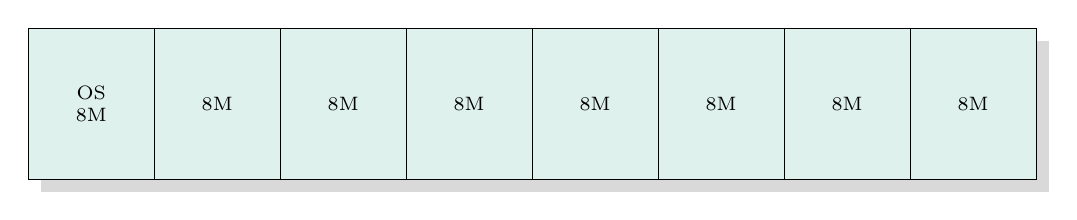
\begin{tikzpicture}[scale=1.6,font=\scriptsize]
      \fill[gray!30] (.1,-.1) rectangle (8.1,1.1);
      \draw[fill=white!94!blue!93!green] (0,0) rectangle node[align=center]{OS\\8M} (1,1.2);
      \foreach \x in {1,...,7} { 
        \draw[fill=white!94!blue!93!green] (\x,0) rectangle node{8M} ({\x+1},1.2);
      }
    \end{tikzpicture}
    \caption{Particiones iguales.}
  \end{subfigure}

  \vspace{5mm}

  \begin{subfigure}[c]{\linewidth}
    \centering
    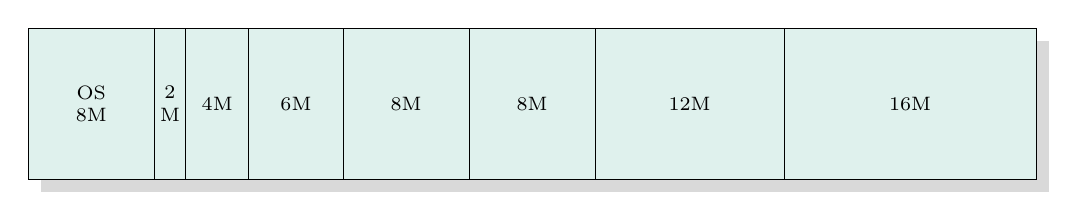
\begin{tikzpicture}[scale=1.6,font=\scriptsize]
      \fill[gray!30] (.1,-.1) rectangle (8.1,1.1);
      \draw[fill=white!94!blue!93!green] (0,0) rectangle node[align=center]{OS\\8M} (1,1.2);
      \foreach \x\d\t in {1/1.25/2\\M, 1.25/1.75/4M, 1.75/2.5/6M, 2.5/3.5/8M, 3.5/4.5/8M, 4.5/6/12M, 6/8/16M} { 
        \draw[fill=white!94!blue!93!green] (\x,0) rectangle node[align=center]{\t} (\d,1.2);
      }
    \end{tikzpicture}
    \caption{Particiones distintas.}
  \end{subfigure}
  \caption{Ejemplo de particiones fijas a una Memoria de 64~Mbyte.}
  \label{fig:particionado_fijo}
\end{figure}

Las particiones de tamaño fijo presentan dos problemas importantes:
\begin{itemize}
  \item Un proceso puede ser demasiado grande para cualquier partición, obligando a utilizar \textit{overlays}\footnote{Overlay: técnica de gestión de memoria en la que un mismo espacio de memoria se utiliza sucesivamente para distintas partes (módulos) de un programa que no se ejecutan al mismo tiempo. Así, aunque el programa no quepa completo en memoria, solo se carga en memoria activa la parte necesaria en cada momento, reduciendo el uso total de memoria.}.
  \item Se produce \textit{fragmentación interna}, ya que un proceso ocupa toda la partición aunque utilice solo una parte de ella.
\end{itemize}

Las particiones de distinto tamaño reducen, pero no eliminan, estos inconvenientes.

\paragraph{Algoritmo de ubicación}

Con particiones de igual tamaño, la asignación es trivial: cualquier partición libre puede alojar al proceso.

Con particiones de distinto tamaño existen dos estrategias:
\begin{itemize}
  \item \textit{Una cola por partición:} cada proceso espera por la partición más pequeña donde pueda ejecutarse. Minimiza la fragmentación interna, pero algunas particiones grandes pueden permanecer sin utilizar.
  \item \textit{Una única cola global:} cuando una partición queda libre, se selecciona el proceso adecuado y se asigna a la partición disponible más pequeña que pueda contenerlo. Este enfoque aprovecha mejor la memoria del sistema.
\end{itemize}

Si no hay particiones libres, el sistema debe seleccionar un proceso para intercambiar (\textit{swap out}), decisión que puede basarse en diversos criterios, como el tamaño de la partición, la prioridad del proceso o su estado (listo o bloqueado).

\begin{figure}[!ht]
  \centering 
  \begin{subfigure}[c]{0.45\textwidth}
    \centering 
    \includegraphics[width=\linewidth]{chapters/05_unit/media/one_queue_per_partition.pdf}
    \caption{Una cola de procesos por partición.}
    \label{fig:una_cola_por_proceso}
  \end{subfigure}
  \hspace{4mm}
  \begin{subfigure}[c]{0.45\textwidth}
    \centering
    \includegraphics[width=\linewidth]{chapters/05_unit/media/one_queue_all_partition.pdf}
    \caption{Única cola.}
  \end{subfigure}
  \caption{Asignación de memoria para particionado fijo.}
\end{figure}

\paragraph{Ventajas y desventajas}

Las principales ventajas del particionamiento fijo son:
\begin{itemize}
  \item implementación sencilla;
  \item bajo costo de administración por parte del sistema operativo.
\end{itemize}
Sin embargo, presenta importantes limitaciones:
\begin{itemize}
  \item el número de particiones limita el número máximo de procesos activos;
  \item la memoria se utiliza de forma ineficiente debido a la fragmentación\footnote{Fragmentación: desperdicio de memoria ocasionado cuando los procesos se alojan en espacios que no quedan perfectamente ajustados. Puede ser interna (memoria dentro de una partición asignada que no se utiliza) o externa (memoria libre total suficiente, pero repartida en ``huecos'' no contiguos, impidiendo asignar un bloque continuo a un proceso).} interna;
  \item los tamaños de las particiones son fijos y no pueden adaptarse a las necesidades de los procesos.
\end{itemize}

Por estas razones, el particionamiento fijo prácticamente ha desaparecido de los sistemas operativos modernos.

\subsection{Particionamiento dinámico}

El \textit{particionamiento dinámico} fue desarrollado para solucionar algunas limitaciones del particionamiento fijo. En este esquema, las particiones no tienen un tamaño predeterminado: cuando un proceso se carga en memoria, se le asigna exactamente la cantidad de memoria que necesita.

\begin{figure}[!ht]
  \centering
  \includegraphics[width=0.8\textwidth]{chapters/05_unit/media/external_fragmentation.pdf}
  \caption{Fragmentación externa por el efecto del particionamiento dinámico.}
  \label{fig:ext_fragmentation}
\end{figure}

Esta técnica elimina prácticamente la \textit{fragmentación interna}, pero introduce un nuevo problema: la \textit{fragmentación externa}. A medida que los procesos terminan o son intercambiados mediante \textit{swapping}, quedan pequeños bloques libres (\textit{huecos}) dispersos en la memoria, como se muestra en la figura \ref{fig:ext_fragmentation}. Aunque la suma de estos espacios libres sea suficiente, puede no existir un bloque contiguo lo bastante grande para alojar un nuevo proceso.

Una solución consiste en realizar \textit{compactación}, desplazando los procesos para reunir toda la memoria libre en un único bloque contiguo. Sin embargo, esta operación consume tiempo de CPU y requiere soporte de \textit{reubicación dinámica} para actualizar las direcciones de memoria de los procesos.

\paragraph{Algoritmos de ubicación}
Cuando existen varios bloques libres capaces de alojar un proceso, el sistema operativo debe decidir cuál utilizar. Los algoritmos más comunes son:
\begin{figure}[!ht]
  \centering  
  \includegraphics[width=0.8\textwidth]{chapters/05_unit/media/algorithms_dynamic_memory.pdf}
  \caption{Configuraciones de la memoria antes y después usando diferentes tipos de algoritmos.}
\end{figure}
\begin{itemize}
  \item \textit{First-Fit}: selecciona el primer bloque libre suficientemente grande. Es el algoritmo más simple y, en general, el más rápido y eficiente.
  \item \textit{Next-Fit}: continúa la búsqueda desde la última asignación realizada. Suele ofrecer un rendimiento ligeramente inferior al de \textit{First-Fit}, ya que tiende a fragmentar la parte final de la memoria.
  \item \textit{Best-Fit}: elige el bloque libre más pequeño que pueda alojar el proceso. Aunque minimiza el espacio desperdiciado en cada asignación, genera numerosos fragmentos pequeños, aumentando la fragmentación externa y la necesidad de compactación.
\end{itemize}

En la práctica, \textit{First-Fit} suele ofrecer el mejor equilibrio entre velocidad y aprovechamiento de la memoria.

\paragraph{Algoritmo de reemplazo}

Si todos los procesos residentes están bloqueados y no existe memoria suficiente para cargar otro proceso (incluso después de compactar), el sistema operativo debe seleccionar un proceso para intercambiar (\textit{swap out}) y liberar espacio.

La elección del proceso a reemplazar depende del algoritmo de reemplazo utilizado, tema que se estudia posteriormente junto con los esquemas de memoria virtual.

\subsection{Sistema Buddy (compañeros)}

El \textit{Buddy System} es un compromiso entre el particionamiento fijo y el dinámico. Busca reducir la fragmentación y evitar el elevado costo de la compactación, manteniendo una administración de memoria relativamente sencilla.

La memoria se organiza en bloques cuyo tamaño es una potencia de dos, es decir, de tamaño \(2^K\), donde:
\begin{itemize}
  \item \(2^L\): tamaño mínimo de bloque asignable.
  \item \(2^U\): tamaño máximo de bloque, normalmente igual al total de memoria disponible.
\end{itemize}
Inicialmente, toda la memoria forma un único bloque de tamaño \(2^U\). Cuando un proceso solicita memoria:
\begin{itemize}
  \item Si existe un bloque libre del tamaño adecuado, se asigna directamente.
  \item Si el bloque disponible es demasiado grande, se divide en dos bloques iguales llamados \textit{buddies} (``compañeros''). El proceso se repite recursivamente hasta obtener el bloque más pequeño cuya capacidad sea suficiente para la solicitud.
\end{itemize}
Matemáticamente, si se realiza una solicitud de tamaño \(s\) tal que \(2^{U-1}<s\leq 2^U\), entonces se asigna todo el bloque. De lo contrario, el bloque se divide en dos compañeros iguales de tamaño \(2^{U-1}\). Este proceso continúa hasta que se genera el bloque más pequeño mayor o igual que \(s\) y se asigna a la solicitud.

El sistema mantiene listas de bloques libres para cada tamaño posible. Es posible que un hueco sea eliminado de la lista (\(i+1\)) dividiéndolo por la mitad para crear dos compañeros de tamaño \(2^i\) en la lista \(i\). Cuando un bloque se libera, si su compañero también está libre, ambos se fusionan para formar un bloque del doble de tamaño. Este proceso puede repetirse recursivamente hasta obtener el bloque más grande posible.

Si se solicita una asignación de tamaño \(k\) tal que \(2^{i-1}<k\leq 2^i\), se utiliza el siguiente algoritmo recursivo para encontrar un hueco de tamaño \(2^i\):

\begin{ccode}[title=Algoritmo recursivo utilizado para encontrar un hueco]
void get_hole(int i) {
  // condición de corte: se ha sobrepasado el tamaño máximo de memoria
  if (i == (U+1)) <fallo>;
  // si hay bloque de orden i, ignora y salta a la línea 10 
  if (<i_list vacía>) { 
    get_hole(i+1); // busca particionar un bloque mayor
    <separar hueco en compañeros>;
    <colocar compañeros en i_list>;
  }
  <tomar primer hueco en i_list>;
}
\end{ccode}

\paragraph{Ventajas}

\begin{itemize}
  \item Administración de memoria simple y eficiente.
  \item La fusión automática de bloques reduce la fragmentación externa.
  \item La asignación y liberación de memoria son rápidas.
\end{itemize}

\paragraph{Desventajas}

\begin{itemize}
  \item Puede producir \textit{fragmentación interna}, ya que los bloques siempre tienen tamaños que son potencias de dos.
  \item Resulta menos flexible y eficiente que los esquemas modernos de memoria virtual basados en paginación y segmentación.
\end{itemize}

\begin{figure}[!ht]
  \centering
  \includegraphics[width=0.9\textwidth]{chapters/05_unit/media/buddy.pdf}
  \caption{Ejemplo de asignaciones del sistema Buddy.}
\end{figure}

Aunque hoy en día rara vez se utiliza como mecanismo principal de administración de memoria, el \textit{Buddy System} continúa empleándose en algunos sistemas, como la asignación de memoria del kernel de UNIX y en sistemas paralelos.

\subsection{Reubicación}

En los esquemas donde un proceso siempre ocupa la misma partición (por ejemplo, particiones fijas con una cola por partición --- Figura \ref{fig:una_cola_por_proceso}), basta con utilizar un cargador reubicador (un proceso siempre vuelve a la misma partición). Al cargar el proceso por primera vez, todas las direcciones relativas del programa se convierten en direcciones físicas absolutas según la dirección base de la partición asignada.

El problema aparece cuando un proceso puede ocupar particiones distintas durante su vida (particiones de igual tamaño, una única cola para particiones desiguales o particionamiento dinámico), ya que las direcciones absolutas dejan de ser válidas. En estos casos las posiciones de instrucciones y datos no son fijas, ya que cambian en cada \textit{swap-in} o desplazamiento durante la compactación.

Para resolverlo se distinguen dos tipos de direcciones:
\begin{itemize}
  \item \textit{Dirección lógica:} referencia independiente de la ubicación física del proceso.
  \item \textit{Dirección relativa:} caso particular de dirección lógica, expresada como un desplazamiento respecto de un punto conocido (generalmente el inicio del programa).
  \item \textit{Dirección física/absoluta:} ubicación real en memoria principal.
\end{itemize}

Los programas se cargan utilizando reubicación dinámica en tiempo de ejecución (\textit{dynamic run-time loading}) con soporte de hardware, manteniendo las referencias como direcciones relativas. Durante la ejecución, el hardware traduce automáticamente cada dirección relativa a una dirección física.

Cuando un proceso pasa a estado \textit{Running}, se cargan dos registros especiales (Figura~\ref{fig:soporte_hw_realocation}):
\begin{itemize}
  \item \textit{Registro base:} contiene la dirección inicial del proceso en memoria.
  \item \textit{Registro límite:} contiene la dirección final de datos (inicio de pila).
\end{itemize}
\begin{figure}[!ht]
  \centering
  \begin{tikzpicture}[>=Stealth,font=\scriptsize]
    \fill[fill=gray!20] (0.1,-0.1) rectangle (2.1,5.4);
    \draw[fill=white!94!blue!93!green] (0,0) rectangle node{Pila} (2,1);
    \draw[fill=white!94!blue!93!green] (0,1) rectangle node{Datos} (2,3);
    \draw[fill=white!94!blue!93!green] (0,3) rectangle node{Programa} (2,5);
    \draw[fill=white!94!blue!93!green] (0,5) rectangle node{PCB} (2,5.5);

    \node[
      fill=gray!15,
      draw,
      rectangle
      ] (adder) at (-3,4) {Sumador};
    \node[
      fill=gray!15,
      draw,
      rectangle
      ] (comp) at (-3,3) {Comparador};
    \node[
      fill=gray!15,
      draw,
      rectangle
      ] (br) at (-6,5) {Registro Base};
    \node[
      fill=gray!15,
      draw,
      rectangle
      ] (lr) at (-6,3) {Registro límite};
      
    \draw[thick,->] (4,6.5) coordinate(tmp) -- node[above]{Dirección Relativa} (tmp -| adder) -- (adder);
    \draw[thick,->] (adder) -- node[right]{Dirección absoluta} (comp);
    \coordinate (datos) at (0,2);
    \draw[dashed,->] (comp) -- ++(2,0) coordinate(tmp) -- (datos -| tmp) -- (0,2);
    \draw[dashed,->] (comp) -- ++(0,-.8) node[below]{Interrupción al SO};
    \coordinate (pstack) at (0,1);
    \draw[dashed,->] (lr) -- (pstack -| lr) -- (pstack);
    \draw[dashed,->] (br) -- (0,5);
    \draw[thick,->] (br) -- (adder -| br) -- (adder);
    \draw[thick,->] (lr) -- (comp);
  \end{tikzpicture}
  \caption{Soporte de hardware para la reubicación.}
  \label{fig:soporte_hw_realocation}
\end{figure}

En cada acceso a memoria la traducción es:
\[
\text{dir}_{\text{física}} = \text{dir}_{\text{relativa}} + \text{base}
\]

Luego se verifica que \(\text{dir}_{\text{física}} \leq \text{bounds}\). Si está dentro de los límites, la ejecución continúa; si no, se genera una interrupción al SO.

Este mecanismo permite intercambiar y mover procesos libremente y, a la vez, proporciona protección y aislamiento entre procesos.

